\begin{figure}[!htp]
    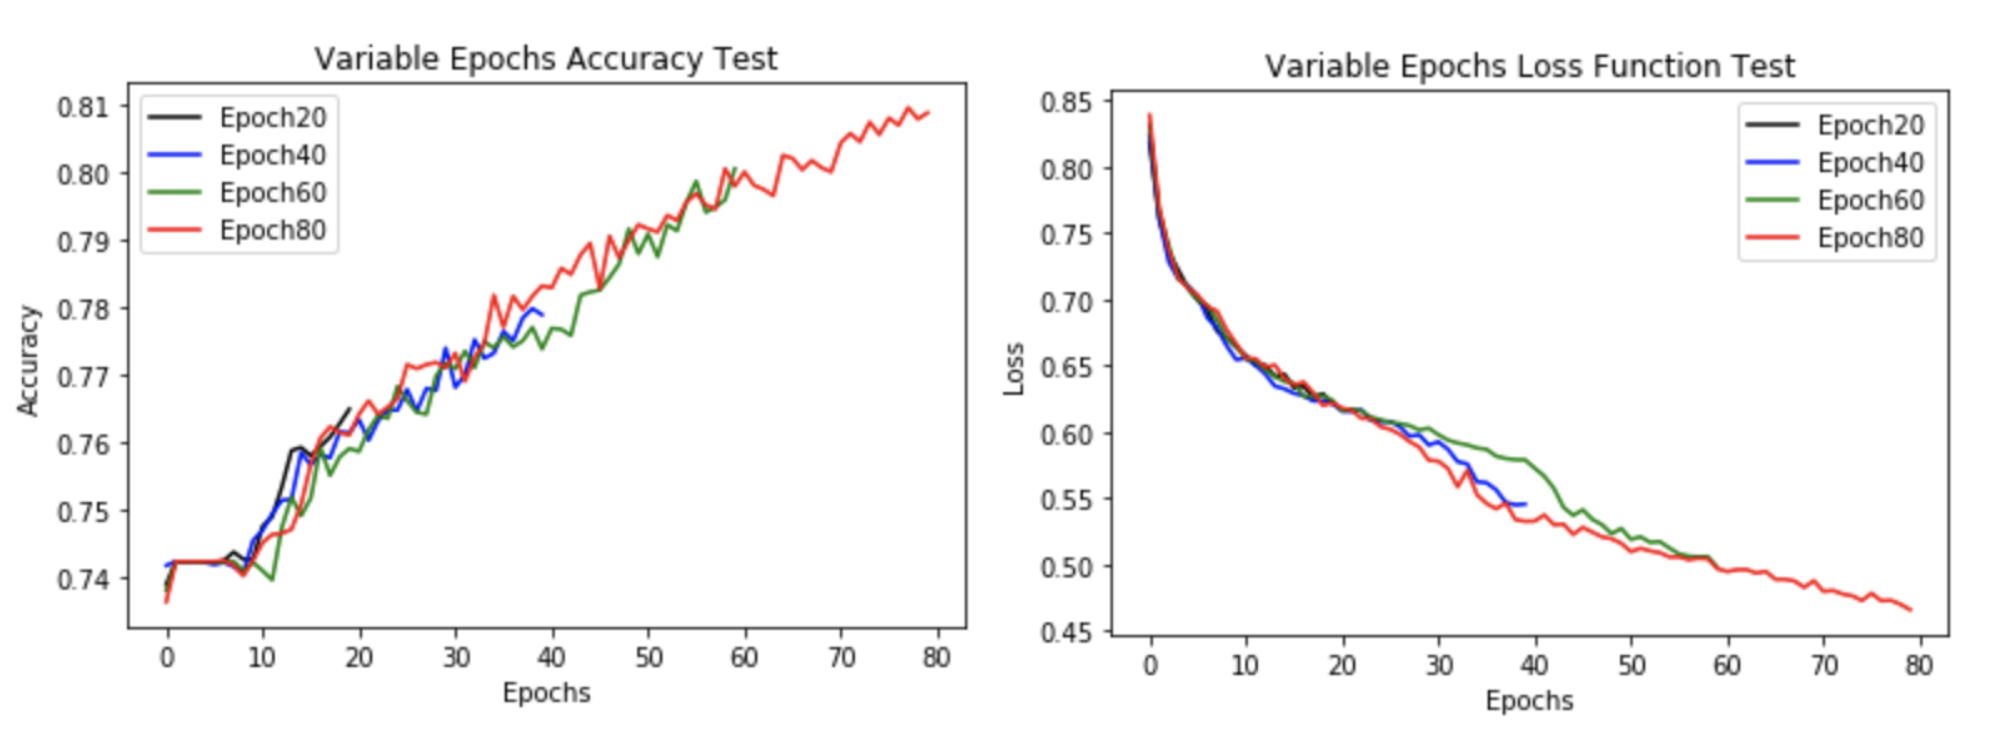
\includegraphics[width=\textwidth]{Images/epochs.png}
    \caption{Results obtained different epochs}
    \label{fig:epochsTest}
\end{figure}

The figure \ref{fig:epochsTest} shows the accuracy of model with same architecture for 
different number of epochs. The model accuracy is directly proptional the number of epochs as 
training the nural networks is optimisation problem and objective is to find minimum of the cost 
function. The model accuracy on training data improves over each epoch as the model finds 
local minimum of cost function at each epoch and improve the predection in the next iteration.
However, when the model reaches the gloabal minimum of the objective function there will 
be improvments in model accuracy. The figure \ref{fig:epochsTest} shows the model trained 
with the most number of epochs which is eighty in these experiments has least value of 
cost function and maximum training accuracy.

\begin{center}
    \begin{tabular} { | c | c | c | c |}
        \hline
        Learning Rate & Test Accuracy & Epochs  & Optimiser\\ 
        \hline
        0.01 & 73.61\% & 20 & SGD \\ 
        \hline 
        0.01 & 76.97\% & 40 & SGD  \\
        \hline 
        0.01 & 79.46\% & 60 & SGD \\
        \hline
        0.01 & 78.68\% & 80 & SGD \\
        \hline
    \end{tabular}
\end{center}

The table above shows the results obtained from evaluating model accuracy on the test data trained 
over different number of epochs. The general trend can be observed that with the increase in the epochs 
model accuracy was also observed to be improved. 